\documentclass{report}
\usepackage[utf8]{inputenc}

\title{Plutt: Strict Type Checking, Semantic Versioning, and Location Transparency in Micro Front-end Components}
\author{Julius Celik \texttt{<jcelik@kth.se>}}
\date{\today}

\usepackage[euler]{textgreek}

\setlength{\parindent}{0em}
\setlength{\parskip}{1em}

\usepackage{biblatex}
\addbibresource{references.bib}

% For acronyms in the text
\usepackage[printonlyused]{acronym}

% For images
\usepackage{graphicx}

% For blockquotes
\usepackage{csquotes}

\usepackage{enumitem}

% For subfigures
\usepackage{subcaption}

% For code blocks
\usepackage{listings}


\begin{document}

\maketitle

\setlength{\parskip}{0em}
\tableofcontents
\setlength{\parskip}{1em}


% \begin{acronym}
% \acro{DX}{Developer Experience}
% \acro{UX}{User Experience}
% \end{acronym}
% 
\chapter{Introduction}

\section{Background}
\acp{MFE} is a web \ac{FE} architecture style, where the \ac{FE} is composed of multiple simultaneously running applications. As the name implies it is heavily inspired by the microservice architecture style. It promises \ac{DX} improvements similar to those that microservices provide, like team independence, clear code responsibility, and high cohesion. Additionally \acp{MFE} promises a higher cohesion between \ac{BE} and \ac{FE}, mitigating feature latency that comes from asynchronous deployment. In practice this means that the delay from starting to implement a feature to it reaching market, should be decreased when using \acp{MFE} \cite{Celik}. \textbf{ADD SOURCES!!!}


\section{Problem Statement}

Write about how teams should be very divided and independent

Write about how teams would like to try \ac{MFE} but should not edit code from other teams.

\section{Problem}

Is it possible to implement \ac{MFE} without changing other parts of the code base? Access transparency and self contained micro frontends. Three artifacts are introduced:

\begin{description}
\item[Construct] Self contained micro frontends.
\item[Instantiation] Plutt -- A build tool for self contained micro frontends.
\item[Method] The method of creating self contained micro frontends.
\end{description}


\textbf{Old problem}

The feasibility of \acp{MFE} are unknown, as the performance impacts are not known. It is believed that \ac{DX} could be improved by using \acp{MFE}, but the technology is criticised for possibly introducing a large negative performance impact, which in turn affects \ac{UX}.


It would be interesting to measure the \ac{UX} performance impact when using \acp{MFE}. If it could be shown that a complex production facing web application could be transformed, to use a \ac{MFE} architecture \textit{without} a significant performance impact, the criticism regarding performance can be rejected. The problem can be condensed into the following research question:

\begin{center}
\begin{tabular}{p{0.28\textwidth}p{0.60\textwidth}}
     \textbf{Research Question:} & Is it possible to transform a monolithic complex production facing web application, to use a \ac{MFE} architecture, without \ac{UX} being significantly affected?
\end{tabular}
\end{center}

\section{Hypothesis}
It is possible to implement a monolithic complex web application using a \ac{MFE} architecture, without a large negative impact on performance and \ac{UX}.

\section{Purpose}
The purpose is to evaluate the feasibility of using \acp{MFE}, regarding \ac{UX}. The impact on \ac{DX} will not be evaluated. Assuming that \ac{DX} is positively impacted, there is a value in knowing if there is a trade-off between \ac{DX} and \ac{UX} or if \ac{UX} impacts are negligible.

\section{Goal}
The goal is to try to transform a monolithic complex web app, to using a \ac{MFE} architecture and compare performance between the monolithic web page and the \ac{MFE} web page. The attempt is that the \ac{MFE} page will have similar performance to the monolithic page, as this would mean that only \ac{DX} has to be considered when evaluating the use of \acp{MFE}.

\section{Tasks}
Initially a literature study will be conducted with two purposes:

\begin{enumerate}
    \item Evaluate the different methods for implementing a \ac{MFE} architecture.
    \item Decide on quantifiable performance metrics that have shown an impact on \ac{UX}. Likely metrics could be bundle size, time to first interaction, or time to first render. As there exists extensive research into this field, the chosen metrics will be a very trustworthy measurement of \ac{UX} impact.
\end{enumerate}

When an implementation and evaluation method is chosen, a complex monolithic web application will be re-implemented, using a \ac{MFE} architecture. When the modified web page is created the original and modified page can be compared, using the chosen performance metrics.

Finally the results will be evaluated and analyzed. The research question will be answered. All of this will be compiled into the thesis.

\section{Research Methodology}

\section{Old Method}
The project will use an empirical method. There exists quantifiable measurements, and the correlation between these and \ac{UX} are very extensively proven. Therefore, there exists a good foundation for conducting performance tests on web pages, and then from analysis of these measurements deduce \ac{UX} impact.

The biggest flaw with the chosen method is that it does not provide any method for proving that \acp{MFE} lead to a negative \ac{UX} impact. If the modified page is significantly worse than the original page it only proves that this specific page became worse, which could be because of a poor implementation. If the modified page has similar performance as the original page it proves that it is possible to create a \ac{MFE} web page with no significant performance degradation. Therefore, the hypothesis can be proven, but not rejected.

\section{Supervisor and Examiner}

My supervisor from KTH will be Martin Monperrus. My examiner from KTH will be Benoit Baudry.

The project will be conducted at DigitalRoute who will provide Tommy Gunnarsson as a supervisor. They will also provide me with any necessary equipment like a computer, and access to all of the development tools used at DigitalRoute.

\section{Eligibility and study planning}

All my courses from my bachelor are completed. I have completed more than 60 credits of advanced courses in my master. During my master thesis, I will conduct one 7.5 credit course, and after my master thesis I will have finished all courses for my master.

\section{Milestone chart}

The project will start on 13 January and end on 29 May. There will be the following milestones:

\textbf{7 February:} The project plan and literature study is finished. At this stage the method for implementation and performance evaluation will be chosen.

\textbf{17 April:} The modified web page will be finished. At this stage performance tests can be conducted.

\textbf{15 May:} The first draft of the Thesis will be finished. If it is accepted a thesis presentation date can be chosen.

\textbf{22 May:} The project presentation has been conducted and peer reviews have been provided.

\textbf{29 May:} The final thesis report is submitted.

\chapter{Background}

\textbf{TODO introduce chapter}

\textbf{lorem ipsum}

\textbf{Maybe mention transparencies somewhere}

\section{HTLM and the DOM}

Web pages are composed of \ac{HTML} and \ac{CSS} documents. \ac{HTML} and \ac{CSS} are declarative programming languages that define the content and styling of web pages \cite{Lie1999}. This means that the \ac{GUI} of a web page is defined by the content of the corresponding \ac{HTML} and \ac{CSS} documents. As \ac{HTML} and \ac{CSS} can be seen as being complementary technologies, and is often used together, all uses of \ac{HTML} will be a reference to both \ac{HTML} and \ac{CSS} for the rest of the thesis. \ac{HTML} was both meant to be written by humans, and generated by computer applications (front-end applications) \cite{Lie1999}. The process of when a front-end application generates \ac{HTML} documents is called rendering.

Front-end applications can be categorized into 5 categories, which are presented in Figure \ref{fig:fe-render-methods}. They are categorized on when, and how close to the client device, the rendering process is executed. Static \ac{HTML} is when a developer manually writes \ac{HTML}. Pre-rendering is when a developer uses another markup language than \ac{HTML}, and then uses a tool to render the markup into \ac{HTML}. The server in this case, where the render is performed, does not necessarily have to be the same server that serves the \ac{HTML} to clients. It is used to describe a computer that is not the client. Pre-rendering is done either for a simpler development process, or for use cases that require a larger feature set than static \ac{HTML} can provide. Server Side and Client Side Rendering is when \ac{HTML} is rendered in run time, which is often done for dynamic content or interactive behaviour. Different rendering methods can be mixed for different parts of a web page. If both server side and client side rendering is used for the same parts, it is called Isomorphic rendering.

\begin{figure}
    \centering
    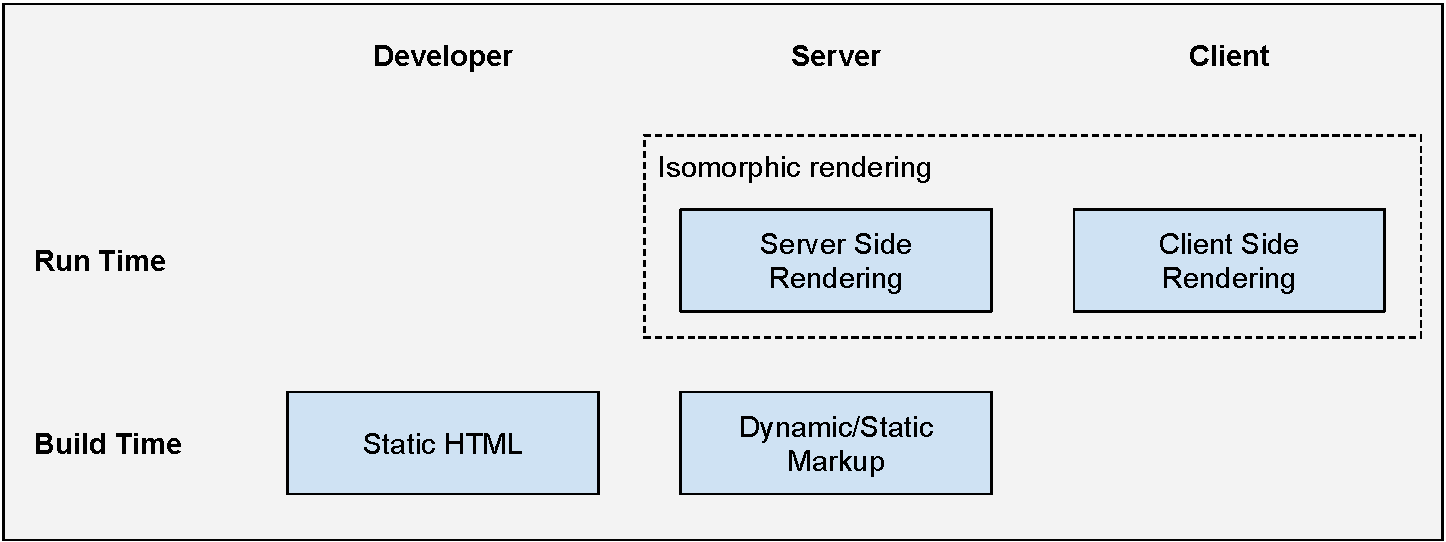
\includegraphics[width=\linewidth]{images/fe-rendering.pdf}
    \caption{Different methods for generating \ac{HTML}. When it is done by a server or client device it is called rendering. Multiple methods can be used for the same web page, and if it is done using different methods, for the same part of the page, it is called isomorphic rendering.}
    \label{fig:fe-render-methods}
\end{figure}

\subsection{Pre-rendering and Server Side Rendering}

Pre-rendering static markup is when tools are used that transform files from one markup format into \ac{HTML}. This is often done in build-time. Pandoc is a tool that translates simpler markdown formats to \ac{HTML} \cite{Dominici2014}. The most prominent benefit is that more lightweight markup languages can be quicker and easier to use when developing web pages as they are more human readable and less verbose, at the cost providing a more limited feature set \cite{Dominici2014}.

There also exists markup languages like PHP that provide a larger feature set than \ac{HTML}. These can provide imperative programming constructs that allow access to perform network calls, composition of reusable components, or resolve database queries \cite{Royappa2000}. These front-end applications can execute their render both in build-time or run-time, depending on if they have to provide dynamic content based on the client request. Dynamic refers to the dynamic nature of the content, where the content is mutable, persistent or user customized. If the render is executed in build time it is pre-rendering based on dynamic content, and if it is done in run time it is called server side rendering.

\subsection{Client Side Rendering}

A front-end application can also be client based where a client receives one or many scripts, that manipulate the \ac{HTML} document. This results in \textit{interactive} applications where user interactions result in animations or GUI changes, without a page refresh. To facilitate this, browsers expose an API, called \ac{DOM}, that allows scripting languages to access and manipulate \ac{HTML} documents \cite{Apparao1998}. This is most commonly done using JavaScript. Already in the beginning of the 2000's researchers experimented with client side rendering, where JavaScript was used to update the \ac{GUI} without a page refresh \cite{Betz2000}.

\textbf{AJAX and asynchronous updates.}

Client side rendering can also be used to render all of the content of a web page, and even simulate page navigation by re-rendering most or all of the web page. This type of front-end application is called \ac{SPA}, because of how the full front-end application is included in one page \cite{Mesbah2007}. Sometimes the different navigation methods are called hard and soft navigation, where soft navigation is when the navigation is simulated by a client side front-end application.

All different front-end applications methods can be mixed where different parts of the \ac{HTML} document is rendered using different methods. If the same parts are rendered both by the server and the client, it is called \textit{isomorphic rendering} \cite{Brehm2013} or universal application \cite{alabes2017isomorphic}. The concept is that a web page is first rendered at the server, sent in a rendered state to the client, and then a replica of the front-end application is sent to the client. When the replica has been loaded on the client, the web page is re-rendered and acts as a traditional \ac{SPA}. The benefit compared to a traditional \ac{SPA} is that the web page is loaded quicker, as the initial file contains all required \ac{HTML} to show the web page \cite{Brehm2013}. It also improves search engine performance, and allows users to optionally use JavaScript\cite{Brehm2013}.

\section{Modern web development}
\subsection{Patterns}
\textbf{discuss modern web applications. Props down, events up. One way data flow}
\subsection{Tools}
\textbf{react/vue, webpack/babel, node, npm/package.json, typescript}

\section{Component Composition}

\textbf{Write about all kinds of approaches to compose a gui of multiple components. Preferably in run time.}

\textbf{Portlets and Mashlets (web mashups)}

\textbf{Transclusion}

\section{Microservices (this section will be re-written)}

\textbf{Focus more on what microsercvices are. The definition.}

Microservices is a software development method where systems are divided into smaller parts, called microservices, that can be individually deployed \cite{Newman2015a}. In turn, this enables low coupling, high cohesion, and strong composability \cite[ch.~1]{Newman2015a}. It also enables multiple developers to work on a shared codebase while minimizing obstruction, which becomes more notable in larger systems, with a large number of developers \cite{Newman2015a}. This concept is also referred to as team independence.

% Microservices are focused on performing single tasks really well, and implementing functionality by composing multiple microservices.

A central aspect of microservices is the concept of ``vertical slicing'' as a decomposition strategy, which is an important facilitator of team independence \cite{Familiar2015}. An example of vertical slicing can be seen in Figure \ref{fig:vertical-slicing}. An early adopter of vertical slicing was \citeauthor{Ratner2011} who observed agile teams who broke up user stories into multiple horizontal layers. They observed that teams focused on one part of the technology stack at a time, which resulted in stories that provided non user facing changes. Vertical slicing solves this by defining stories and responsibilities that encompass end-to-end functionality. This means that instead of thinking in terms of user interface, business logic, and data storage as separate distinct horizontal layers, a story should include all of them, but only from a narrow context \cite{Ratner2011}. \citeauthor{Ratner2011} describes their method as \blockquote{[...] driving a thin vertical slice from UI to database, which is functionally coherent and demonstrable, then progressively widening it with consecutive slices. \cite{Ratner2011}}

\begin{figure}
    \centering
    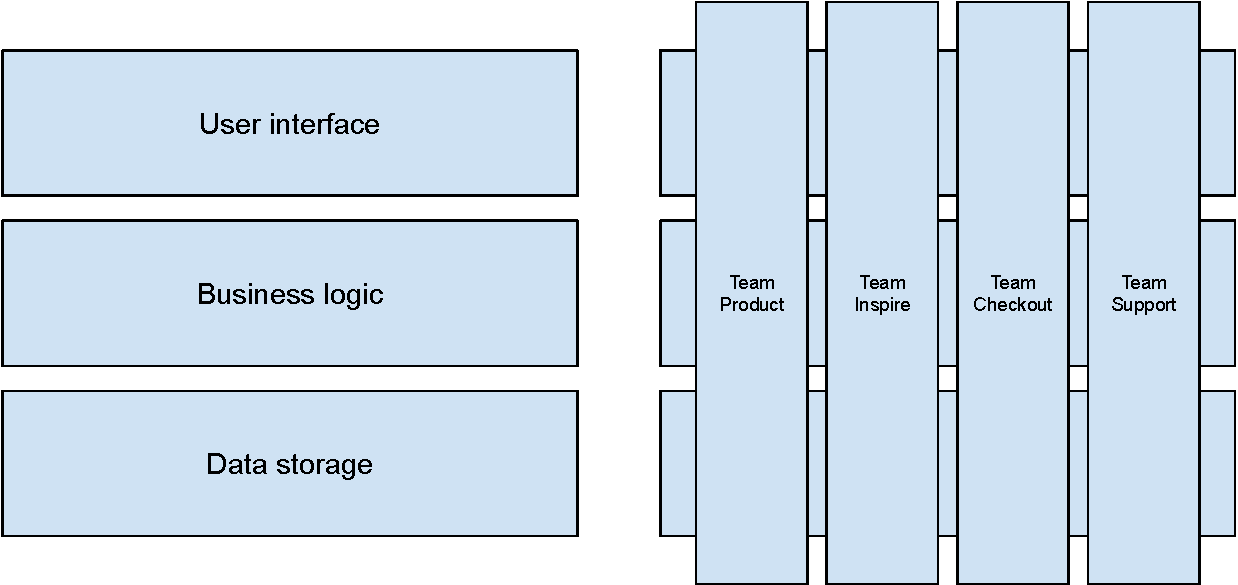
\includegraphics[width=\linewidth]{images/vertical-slicing.pdf}
    \caption{Horizontal Layering and Vertical Slicing. This is an example of four cross functional development teams that are responsible for all aspects of delivering a customer facing feature.}
    \label{fig:vertical-slicing}
\end{figure}

Vertical slicing can be applied to stories like \citeauthor{Ratner2011} describe \cite{Ratner2011}, to team responsibilities, and to system design \cite{Geers2020}. Vertical slicing is a consequence of cross functional agile teams \cite{Geers2020}, which can be explained by Conway's law: \blockquote{Any organization that designs a system (defined broadly) will produce a design whose structure is a copy of the organization's communication structure \cite{Conway}.} This can be interpreted as vertical slicing of system components being a consequence of smaller cross functional teams.

\section{Semantic Versioning and Lock-step Deployments}

See page 64-65 in ``Building Microservices (Sam Newman)''

Gradual Migration

\section{Vertical Decomposition and Self-Contained Systems}
\chapter{Related work}


\section{Micro Front-ends}

Micro front-ends is a front end technique that originates from microservices \cite{Jackson2019}. Where microservices aim to solve scalability problems in the back-end, micro front-ends aim to solve the same problems in the front-end, by applying many of the same concepts and methods. There does not exist one single definition, but one of the introducers of micro front-ends, ThoughtWorks, defines micro front-ends as: \blockquote{An architectural style where independently deliverable front-end applications are composed into a greater whole \cite{Jackson2019}}

An essential common aspect, between microservices and micro front-ends, is the possibility for independent deployability \cite{Jackson2019}, where teams can deploy any changes to software owned by them, without having to coordinate with other teams. The way this is achieved is by using vertical slicing, a software decomposition strategy, based on composing software in functionally coherent slices that fully implement features \cite[ch.~1]{Geers2020}. Using vertical slicing aims to limit the boundary surface areas between different teams' code. Some of the promised benefits of using micro front-ends are simple decoupled codebases, independent deployment, autonomous teams \cite{Jackson2019}, and better customer focus \cite[ch.~1]{Geers2020}.

\citeauthor{Geers2020} presents the evolution of decomposition strategies as in Figure \ref{fig:evolution-of-decomposition-strategies}. Monoliths means that an application is fully included in one code base, and process. An intuitive decomposition is to decompose the front-end from the back-end, which leads to front-end developers being able to work more independently from the back-end. When teams grow it has become more common to divide the monolithic back-end into a vertically sliced microservice back-end. \citeauthor{Geers2020} proposes that it is a natural progression to continue the progress into vertical slices that spans both the back-end and the front-end, which are micro front-ends \cite{Geers2020}.

\begin{figure}
    \centering
    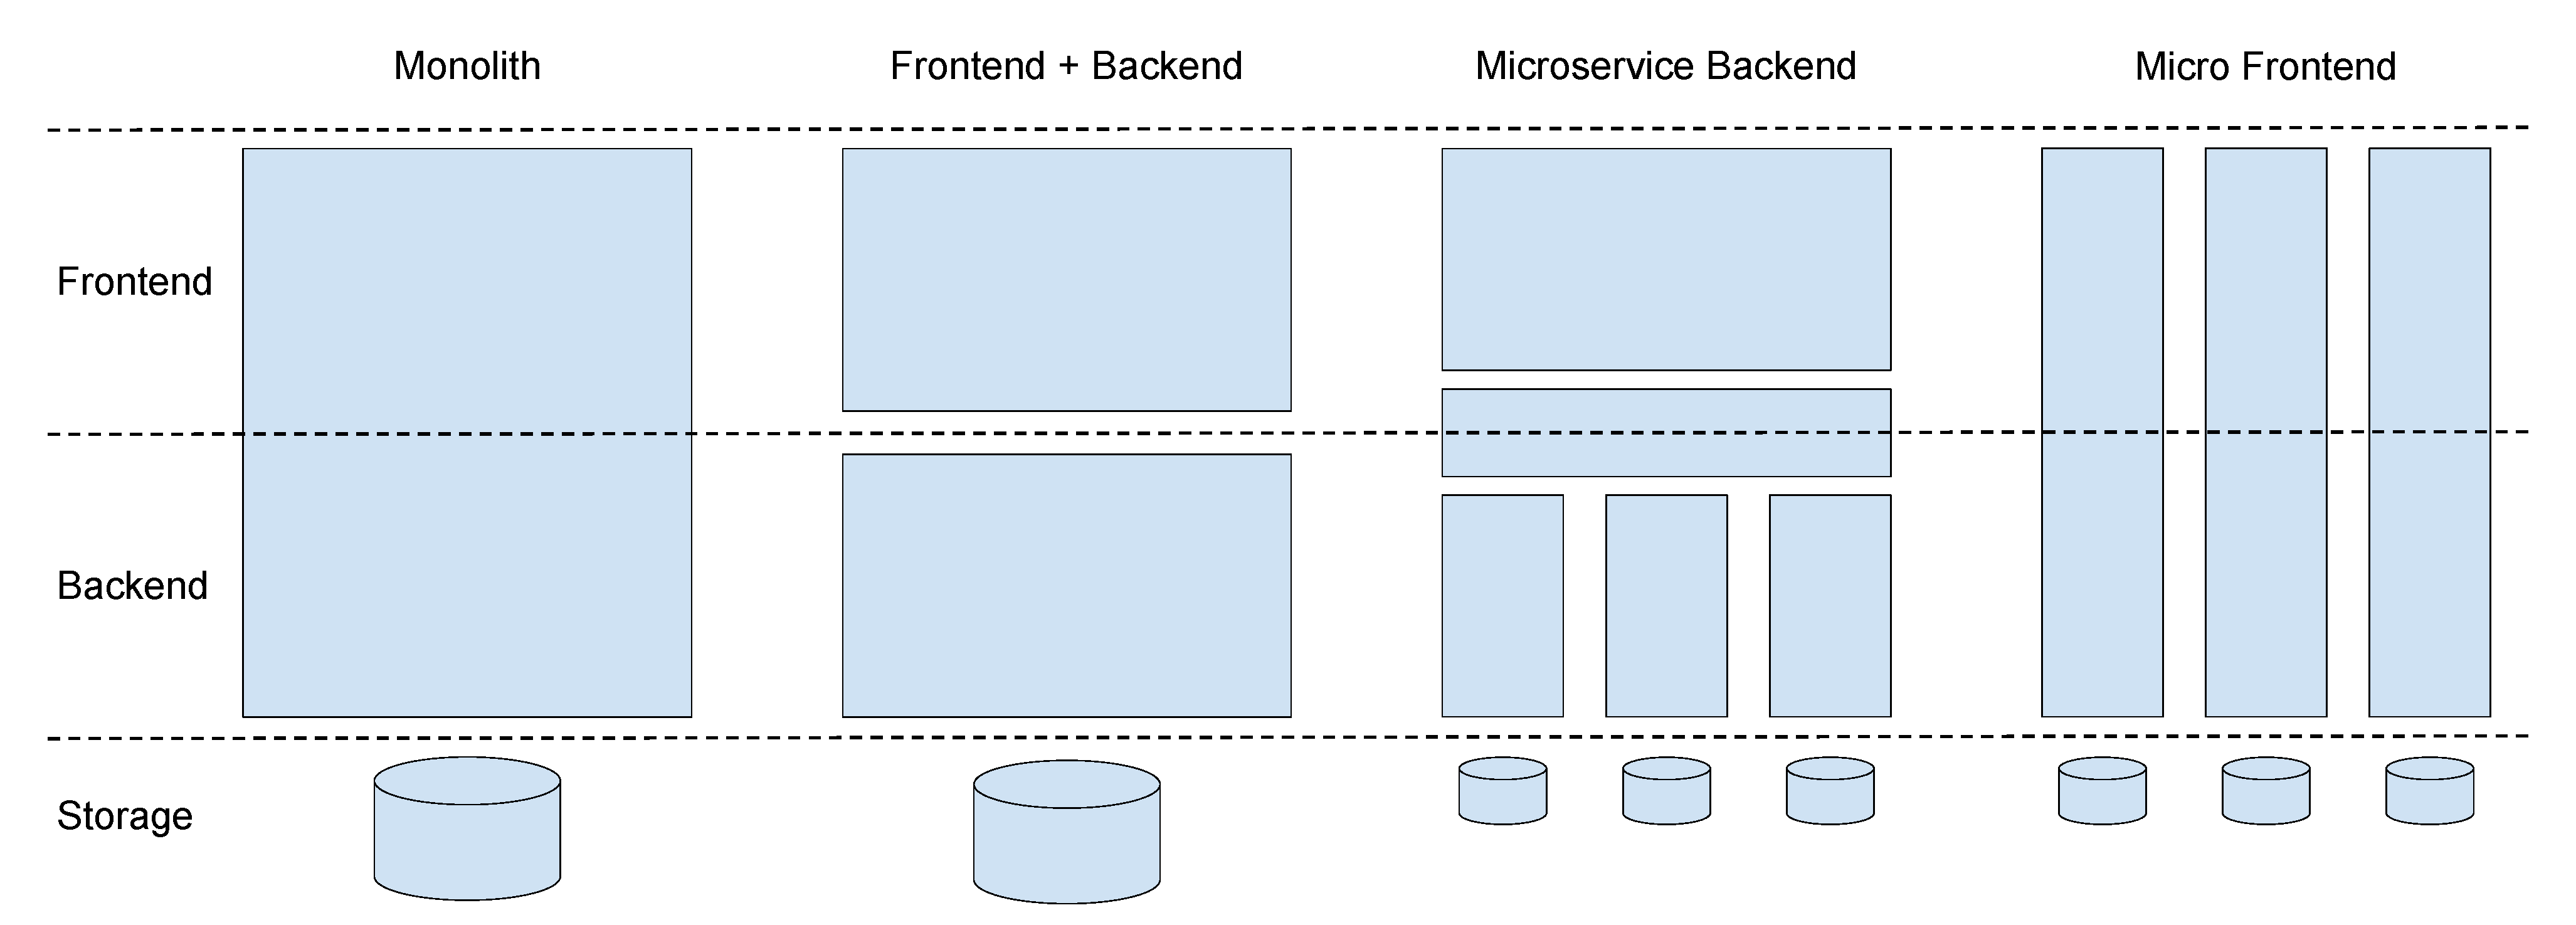
\includegraphics[width=\linewidth]{images/evolution-of-decomposition-strategies.pdf}
    \caption{An Evolution of Decomposition Strategies}
    \label{fig:evolution-of-decomposition-strategies}
\end{figure}

Even though \citeauthor{Geers2020} preferably envisions micro front-ends as fully vertically aligned with the back-end, that does not have to be the case. Many micro front-ends exist apply the architecture patterns of microservices, without being fully aligned with the back-end. Figure \ref{fig:micro-frontend-alignment} presents three approaches to aligning a micro front-end to a back-end. A \textit{Shallow Micro Front-end} is a micro front-end that is in no way aligned to the back-end. The back-end can be one monolith, microservices behind one API-Gateway or multiple services. Based on Conway's law, this probably also means that there exists development teams that work only on the back-end or only on the front-end \cites{Conway}. A \textit{Vertically Aligned Micro Front-end} is when there is a dedicated back-end service that the micro front-end primarily communicates with. A \textit{Monolithic Micro Front-end} is when a micro front-end is a part of a server side rendered monolith, where the back-end and front-end is delivered in one monolithic application. These

\begin{figure}
    \centering
    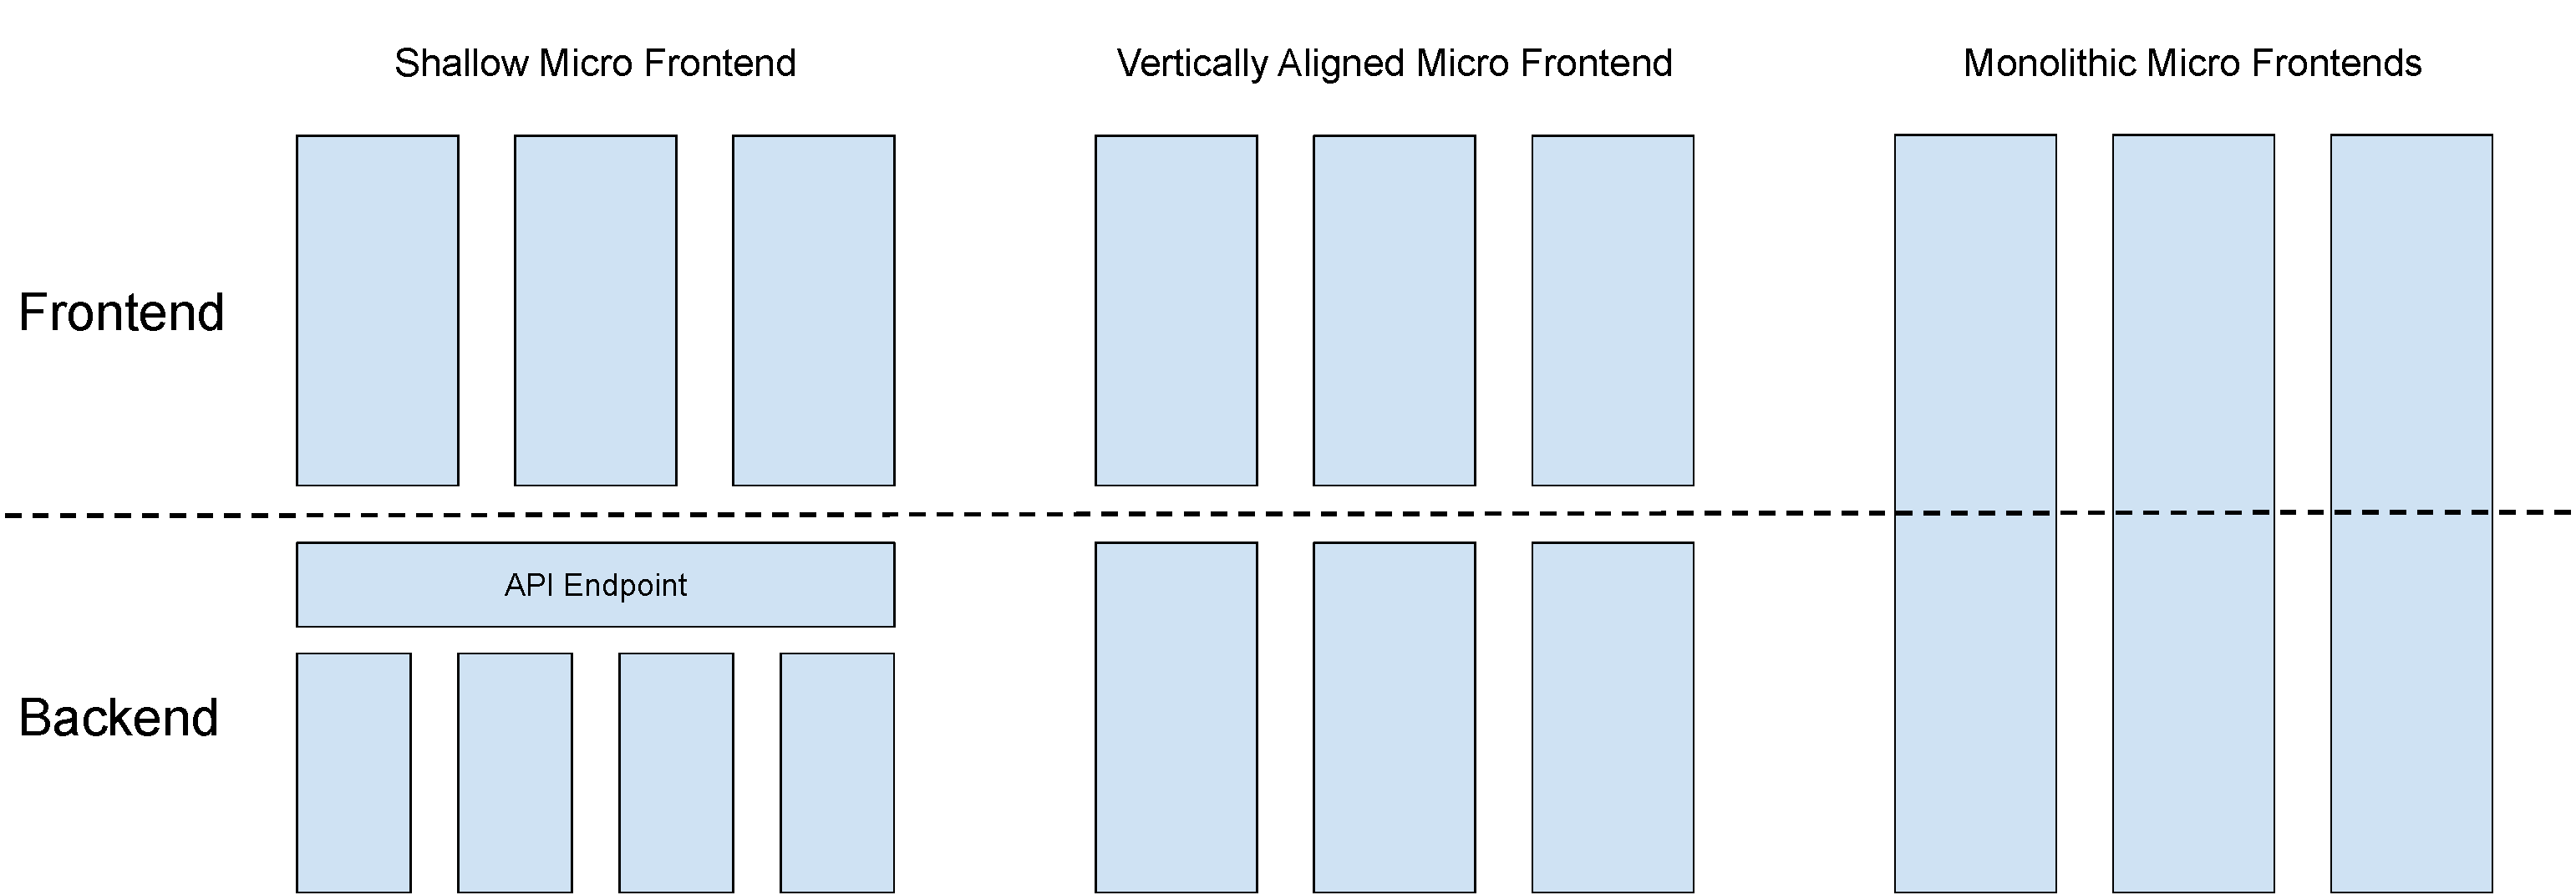
\includegraphics[width=\linewidth]{images/micro-frontend-strategies.pdf}
    \caption{Micro Front-end strategies}
    \label{fig:micro-frontend-alignment}
\end{figure}


\section{Pages and Fragments}

There are many different methods for composing micro front-ends into one coherent front-end. A very important distinction is also to differentiate between micro front-ends that are \textit{pages} or \textit{fragments}. All front-ends are composed by one or more pages. In this case a page refers to a full application view, that covers the full application window. A user can not view multiple pages simultaneously. A fragment is an element of a page. A fragment can be a button, a navigation bar or any other graphical components. A page can include many fragments.

Figure \ref{fig:fragment-page} exemplifies the concept. In this example, the front-end is composed of two pages, which can be served on two different routes. The pages are composed of fragments, and some of the fragments are identical on both pages.

\begin{figure}
    \centering
    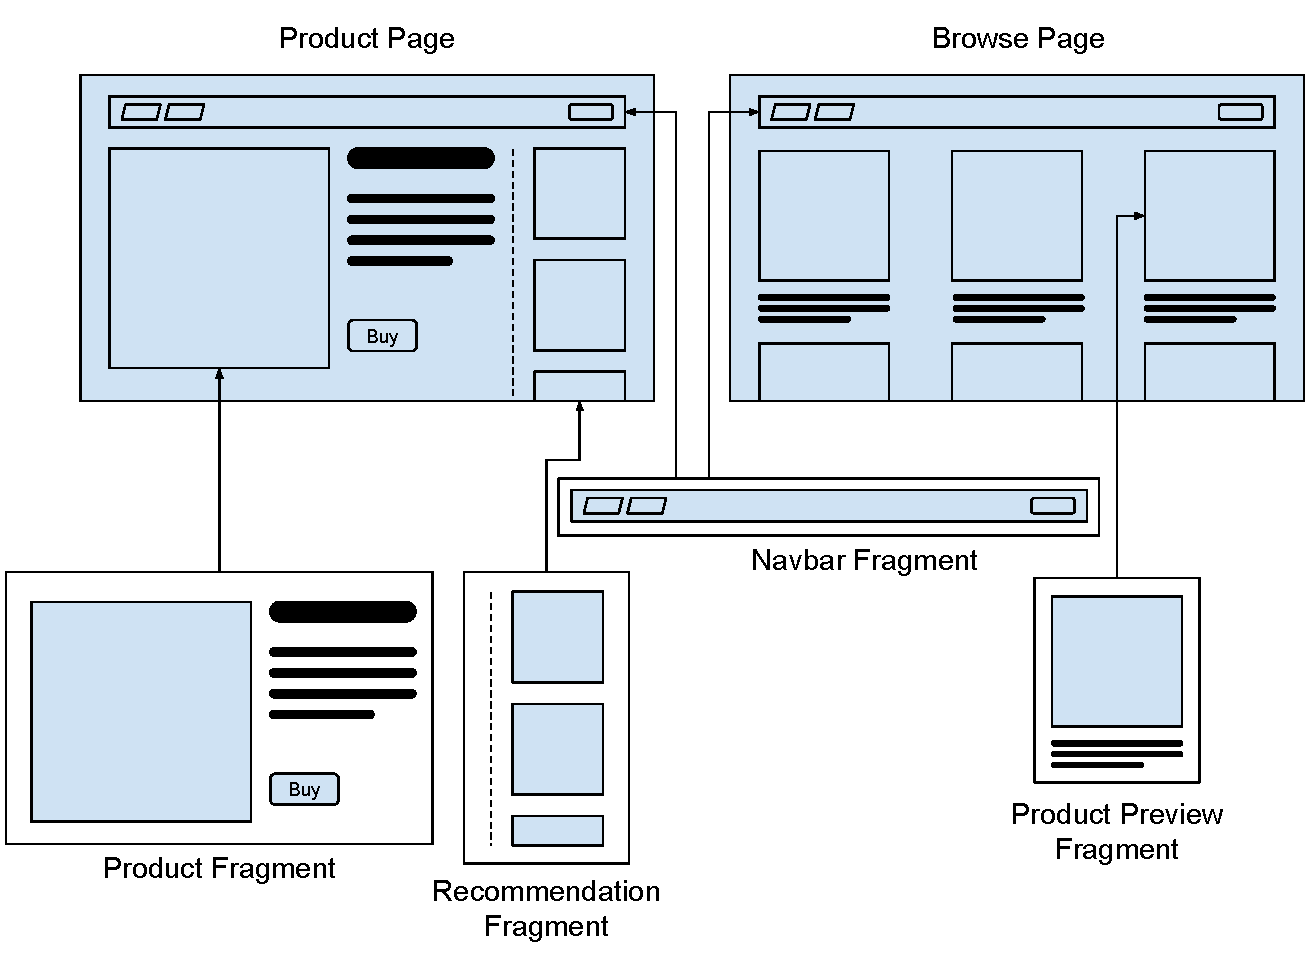
\includegraphics[width=0.9\linewidth]{images/fragment-page.pdf}
    \caption{An example of an e-commerce web page. It consists of two pages, and four fragments, where one fragment is reused on both pages.}
    \label{fig:fragment-page}
\end{figure}

The definition of a fragment is purposefully left vague as ``a part of a page''. The granularity is not specified, which means that multiple fragments in the example could be defined as one fragment, or that a fragment can be divided into multiple fragments. This also implies that a page is an edge case of one large complex fragment.

\section{Composing Micro Front-ends}

As a user uses an application the front-end has to be a coherent application, which means that different micro front-ends has to be integrated into a cohesive experience. Some differentiating questions that arise are ``when and where are the micro front-ends composed?'' The following sections aim to answer those questions. Note that micro front-end \textit{composition} is different from \textit{rendering}, which is when code is evaluated into HTML and CSS code. Composition is the process of integration multiple micro front-ends into one cohesive front-end.

\textbf{mention portlets}

\subsection{When are micro front-ends composed?}

Using ThoughtWorks definition of micro front-ends a micro front-end can be composed both in build-time and run-time \cites{Jackson2019}. Other definitions define micro front-ends as being composed in run-time \cite{Geers2020}. There exists a consensus that using build-time integration loses many of the benefits of using micro front-ends, like independent deployability \cite{Jackson2019}. It is also such a broad definition that most web pages could be defined as micro front-ends. For those reasons, only run-time composition will be considered.

\subsection{Where are micro front-ends composed?}

Micro front-ends can be integrated on the server, on the client, or a combination of both \cite{Jackson2019}. The simplest server side integration is to serve different web pages on different routes \cite{Jackson2019}. All traditional tools and processes can be used to develop the separate pages, and the different micro front-ends can be \acp{SPA}. This can be achieved with a web proxy to serve the different pages on a single domain address, which is visualized in Figure \ref{fig:web-proxy-example}.

\begin{figure}
    \centering
    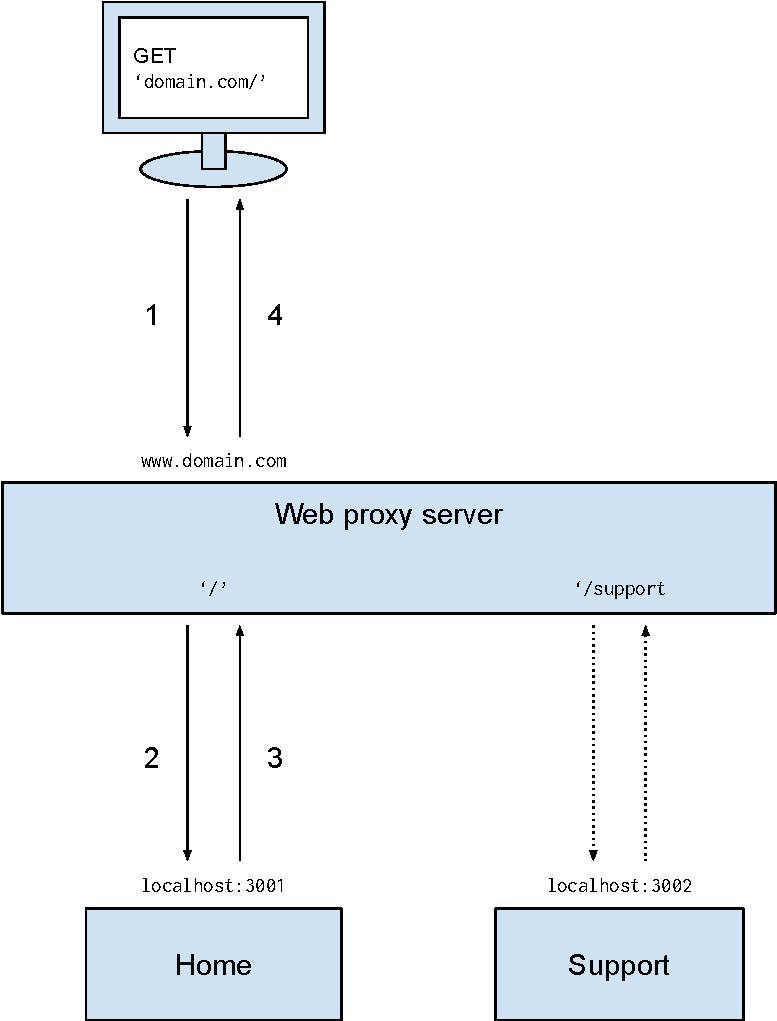
\includegraphics[width=0.5\linewidth]{images/web-proxy.pdf}
    \caption{A web proxy that redirects HTTP requests depending on the route requested. The web servers do can be developed with any existing mature web technology, without having to consider the other servers.}
    \label{fig:web-proxy-example}
\end{figure}

Server side integration can also be used to serve page fragments. This is sometimes called transclusion, and can be done by using technologies like Server Side Includes, Edge Side Includes, Zalando Tailor, or Podium \cite[ch.~4]{Geers2020}. Note that as pages just are large fragments, these technologies can also be used to divide an application on a page level.

All existing client side integration methods can be used for fragment composition, and therefore page composition. The most naive client side integration method is using iframes, which is a web-native standard \cite[ch.~2]{Geers2020}. Iframes were introduced with the HTML 4.01 standard in 1998 \cite{Raggett1999}, when web was still an early technology, which is why there are drawbacks to using them on a modern web app. The most notable trade-offs are performance overhead, accessibility problems, search engine optimization problems, and the lack of layout control \cite[ch.~2]{Geers2020}.

A much newer web-native standard is web components, which in practice is a suite of four web technology standards \cite{MDNWebDocs}. They allow dynamic custom elements to be defined and registered, in an encapsulated scope \cite{MDNWebDocs}. They are used by Google on large products like Youtube to include highly interactive elements \cite{ThePolymerProjectc}.

Figure \ref{fig:web-components} shows an example of how an example web component is created, defined, and what the \ac{DOM} is evaluated into. There are fewer drawbacks with using web components compared with using iframes, but some still exist. The largest issue is that web components do not server side rendering, as they have to be run in a browser at the client \cite[ch.~5]{Geers2020}. This issue can become a problem for performance, accessibility, and search engine optimization. Another drawback, compared with using build-time integration, is the lack of static annotations and analysis. Web components can be internally statically analyzed, but there does not exist any mechanism to share static annotations across the boundary of a web component.

\begin{figure}
\centering
\begin{subfigure}{.65\linewidth}
  \centering
\begin{lstlisting}[
basicstyle=\fontsize{7}{9}\selectfont\ttfamily,
breaklines=true,
frame=single
]
<html>
  <body>
    <my-component></my-component>

    <script>
class MyComponent extends HTMLElement {
  connectedCallback() {
    this.innerHTML = `<h1>Hello!</h1>`;
  }
}

customElements.define(
  'my-component',
  MyComponent
);
    </script>
  </body>
<html>
\end{lstlisting}
  \caption{An example of how to use custom elements. First the class \texttt{MyComponent} is defined, and registered on the name \texttt{my-component}. Then all instances of \texttt{my-component} is replaced on the \ac{DOM} with the custom element \texttt{MyComponent}.}
  \label{fig:sub1}
\end{subfigure}
\hfill
\begin{subfigure}{.30\linewidth}
  \centering
\begin{lstlisting}[
basicstyle=\fontsize{7}{9}\selectfont\ttfamily,
breaklines=true,
frame=single
]
<html>
  <body>
    <my-component>
      <h1>Hello!</h1>
    </my-component>
  </body>
<html>
\end{lstlisting}
  \caption{The result of how the custom element will be evaluated on the \ac{DOM}}
  \label{fig:sub2}
\end{subfigure}
\caption{An example of how to use custom elements which is a part of the Web Component technology suite. The left figure is evaluated to the right figure in run-time.}
\label{fig:web-components}
\end{figure}

As web components are a low-level construct, many frameworks exist that uses web components as a compilation target like Polymer, Stencil, SkateJS, Slim.js, hybrids, and snuggsi \cite{WebComponents.orgb}. Two of the most popular front-end frameworks, Angular \cite{Googlec} and Vue \cite{Vuejs}, has native support for being encapsulated as a web component. The potentially most popular front-end framework React does not natively output web components \cite{Dodson}. However, they do include documentation of how to wrap react components in a web component \cite{FacebookInc.}.

There exists micro front-end meta-frameworks that utilize other technologies than web components. Some of them are simple implementations like react-async-component that creates lazy loaded react components \cite{Matheson}. One of the most popular and extensive frameworks is single-spa \cite{Single-spa}. It is a shell application that includes other applications developed using other frameworks \cite{Single-spa}. Like a thin orchestration layer that handles routing and micro front end composition. This kind of framework has been called a unified single-page application, as it wraps other single-page-applications into one cohesive application \cite{Geers2020}. Single-spa requires that the root application be written as a single-spa application, which implies a considerable migration cost to existing applications \cite{Single-spa}. No micro front-end frameworks provide static analysis between the application boundaries.

\textbf{Summarize all technologies with a figure}

\section{Boundary Pushing Work}

\textbf{I know this is a bad title. What should I call this? It is for work that is being done which is amazing and boundary pushing (will redefine how micro front-ends are used), but not 100\% production ready or public yet.}

Mention Deja vu, Zalandos new framework, Module federation, and portals.
\chapter{Surveying the Industry}
\label{sec:interviews}

A qualitative survey was conducted with five industry experts, to understand how micro front-ends are used in practice and what problems they are applied to. The purpose was to discover aspects that can not be found in existing literature, and compile a common collection of micro front-end knowledge. This contributes to a knowledge base that can be used for developing Plutt and to help other micro front-end research.

\section{Intervied Protocol}

The experts interviewed were chosen based on their contributions to improving micro front-end methodologies or technologies, as well as having an extensive experience in working with micro front-ends. Some were found by their contributions being very public, and others were found recursively by asking the other experts.

To minimize the risk for bias, the questions were standardized. This also made it easier to compare the answers and understand what the experts agreed on and disagreed on. The questions were open ended, and unstructured counter questions were asked to further extract relevant knowledge. The interviews were between 60 and 90 minutes long\footnote{One interview took 4 hours, even though I had planned for 60-90 minutes. A lot of that time was discussing implementation details that is not relevant to the report. So the \textit{relevant} content is about the same as other interviews. Is that noteworthy, or should I just write that the interviews took 60-90 minutes?} and because of large geographical distances they were conducted over video call. They were recorded and can accessed by request.

\subsection{Interviewees}

\begin{description}
    \item[Michael Geers] is a developer who has worked many years for \textit{neuland - Büro für Informatik}. At neuland - Büro für Informatik he has helped large scale e-commerce web pages to use using micro front-ends. Michael is also the creator of \texttt{https://micro-frontends.org/} which at the time of writing is the first google result when searching for \textit{``micro frontends''}, and which is therefore a influential introduction to micro front-ends for many developers. He has been invited to hold talks about micro front-ends on many conferences and is the author of \textit{Micro Frontends in Action} \cite{Geers2020}.
    
    \item[Joel Denning] is a developer who was working on Amazon when he was tasked with solving the problem that their monolithic front-end was a development bottleneck. Inspired by Amazons famous microservice architecture, he developed a micro front-end architecture, which later became the foundation for single-spa. Single-spa is now one of the largest micro front-end composition technologies. He has also worked at Canopy as a front-end team lead until mid 2019, and have since started working as a consultant, helping companies with migrating to and using single-spa.
    
    \item[Luca Mezzalira] was mentioned by three of the other experts as being a central authority in the subject of micro front-ends. As a chief architect and VP of Architecture he has been a vital part of building the architecture for DAZN, a streaming platform with millions of concurrent global users, and hundreds of developers. He regularly speaks at conferences where he promotes the pragmatic micro front-end approach used by DAZN. He is also the author of \textit{Building Micro-Frontends} \cite{Mezzalira2021a}.
    
    \item[Zackary Jackson] has worked as a Senior Frontend Developer at Fiverr and Senior Frontend Architect at Starbucks. At both companies he has worked with refactoring and restructuring the monolithic front-ends into micro front-end applications. He has a background in providing web experiences to users with a slow internet connection, which explains his dedication to minimizing bundle sizes. His work on reducing code duplication lead to him becoming a maintainer of the famous JavaScript module bundler webpack. Zackary introduced the flagship feature for webpack version 5, module federation, which enables micro front-ends to share modules and components, with the primary goal of reducing bundle sizes fetched by client devices.
    
    \item[J\'er\'emy Colin] is a Senior Software Engineer on a Platform Team at \textit{Zalando}. Zalando is famous for their micro front-end suite mosaic, and is often mentioned for being on the forefront of introducing cutting edge micro front-end technologies. J\'er\'emy works with creating their next-generation web architecture, \textit{Interface Framework} \cite{Colin2018}, where parts are heavily inspired from relay \cite{FacebookInc.a}, which J\'er\'emy worked extensively with at \textit{Searchmetrics}. Interface Framework introduces cutting edge concepts like bundling data dependencies together with micro front-end fragments, a recommendation engine that dynamically selects fragments for the optimal user experience, and server side composed isomorphically rendered micro front-ends.
\end{description}

\subsection{Interview Questions}

The questions asked during the interviews where a mix of standardized questions and personalized questions that were related to the interviewees specific contributions and experience. Additional follow up questions were asked for a deeper understanding of the answers. The 12 standardized Interview Questions (IQ) are the following:

{
\setlist[enumerate,1]{label={\textbf{IQ \arabic*}}}
\begin{enumerate}
\item Could you tell me shortly about your experience with micro front-ends?

\item What is your definition of micro front-ends?

\item What would you say that the relation between microservices and micro front-ends is?

\item When should an organization look into using micro front-ends?

\item What are the benefits of micro front-ends?

\item Do you think that micro front-ends provide better UX?

\item How many micro front-ends should a team own?

\item How do you decide on where to place boundaries between micro front-ends?

\item What are your thoughts about team responsibilities when working on a micro front-end architecture? How and by whom is the orchestration handled?

\item Can the orchestration layer include user authentication and other global responsibilities?

\item Where is this field going in the future? What will you be working on?

\item Is there anything else you think I should know?
\end{enumerate}
}

The purpose of the first question was to fully understand the interviewees background, and to understand how that could effect the other questions. To understand what a micro front-end is, and to further understand the point of view of the interviewees answers, IQ 2 and 3 were asked. The later answers differed because the different interviewees had different definitions of micro front-ends, and where therefore discussing different aspects.

IQ 4-6 were meant to understand why micro front-ends are used, and what problems they aim to solve. IQ 7-10 were asked to understand how micro front-ends are and should be used. The last two questions aimed to complement the other questions with anything that was not discussed during the interview.

\textbf{Note: This section could be linked to research questions instead.}

\section{Survey Results}

\subsection{What is a micro front-end?}

The definition is very different when asking different experts, however there were three main aspects that were mentioned, even though not everyone agreed on them. They were independent deployability, isolation, and organizational alignment to business domain.

\textbf{Joel's} definition of micro front-ends is \blockquote{An independently deployable chunk, of your front-end web application.} Joel was humble to that the definition is not fully defined yet, and still evolving, but emphasizes that he believes that independent deployments is the most important aspect, and that build-time integration is a ``monolithic build'' and ``monolithic deployment''. He motivates this both by his definition of microservices, and the reason he thinks micro front-ends are being used:

\blockquote{The problems that micro front-ends solve, are largely organizational problems, not technical problems. And I think that one of the biggest organizational problems that is solved, is [...] different parts of an organization, being able to act independently. Being able to release their code to production without getting approval from everyone else.}

His rough definition of microservices is that microservices are only microservices if they are:

\begin{itemize}
    \item running on a seperate process
    \item communicating via network
    \item independently deployable
    \item have their own data store
    \item have their own build CI/CD process
\end{itemize}
It is impractical or even impossible for micro front-ends to communicate via network, and they are always executed on the same thread. The \ac{DOM}, which can be seen as a replacement for a data store, is shared, which means that they are accessing and mutating the same data store. The remaining technical aspects are independent deployability and separate build processes.

A controversial opinion is that Joel believes there can exist micro front-ends that are non visual. That a micro front-end can provide a service to other visual micro front-ends that are visual.

\textbf{Zackary's} definition is that a micro front-end has to be independently deployable and stand-alone. It was especially important that a micro front-end should work without any dependencies on it's environment, and this is an aspect that contradicts Joel's non visual micro front-ends. Non visual micro-frontends rely on other micro front-ends to update the \ac{DOM}, and if a micro front-end relies on another micro front-end, it is not self contained. Zackary was not against the concept and it's utility, but did not agree on that he would call it a micro front-end.

Zackary mentioned that the back-end is a much easier monolith to break apart into microservices, than the front-end is to break apart into micro front-ends. This relationship is based on that there exists many more technical constraints on the front-end than on the back-end.

\textbf{Michael and Luca's} point of view is much more an organizational. Michael is open to many different definitions but believe that micro front-ends work as a tool to align the back-end with the front-end, using fully vertically aligned teams. Luca does not agree that vertical alignment is necessary, and has a very concrete definition. It doesn't mention visual aspects in any way, and only focuses around organizational aspects. \blockquote{A micro-frontend represents a business domain that is autonomous, is independently deliverable, and is owned by a team.} This definition is very vague from a technological perspective, but is very strict in how they should be applied in an organisation. Both Michael and Luca use \textit{Domain Driven Design} to design their systems.

\textbf{For J\'er\'emy} micro front-ends are an isolated piece of UI. They are isolated in the sense of coupling, and not in the sense of deployments. The most important aspect for J\'er\'emy is that micro front-ends simplifies complexity management. This is very similar to Zackary's point of view, with the exception that J\'er\'emy allows synchronized deployments, and even mono-repositories in his definition.

To summarize, most agree on that microservices is a technical tool to solve an organizational problem. This is done by allowing teams to work more independently. Some believe the independence originates from the strictly decoupled design, while others believe it originates from independent deployments and mostly decoupled design. A micro front-end can possibly be a non-visual component that provides services to other micro front-ends, and that is tied to if the micro front-ends have to be strictly stand-alone or not. Micro front-ends borrow many aspects from microservices, but because of the vastly different execution environments and different constraints, they are also different in many ways. The area of microservice research can be seen as a source of desirable end-results and principles, and not a strict source for specific methods and processes.

\subsection{Why are micro front-ends being used?}

There was a clear consensus that micro front-ends solve complexity problems that arise when there are too many developers working on the same front-end. Solving the scalability problems, can have other indirect positive consequences, like a higher software quality, fewer published bugs, and counterintuitively higher performance. 

Joel was the only interviewee that used microfrontends primarily for ... less code duplication. Michael asset management css bla bla.

\textbf{Michael:} If a monolith is has grown to be too complicated. MFEs gives you a solution to give you clear boundaries. It also gives you a tool to gradually rewrite a large front-end. Like for migrating to a new technology.

For Michael it was always for organizational reasons. For creating vertically aligned teams. The benefit for him is that any time he wants to change or add a feature, he only has to discuss it and align it with one team that owns that feature domain. This is opposite to having to align multiple teams to add or change one feature. Like database, back-end and front-end teams.

A desirable goal is to have as much work and communication as possible being done inside teams, and reducing the need for communication and synchronization between teams.

\textbf{Luca:} Start using at 50 devs.

- Independent deployability

- Fault isolation

- Smaller and easier to work with

- Live support. Quick to do hotfixes.

\textbf{Zackary and Joel:} For a no compromise user experience. Both use micro front-ends to minimize initial bundle load, to maximize metrics like tti or time to first render


\subsection{How are micro front-ends used in practice?}

\textbf{Michael:} Pages are a good division to start with. DDD, and sets of pages are very easy to align with \textit{domains}, with some shared components sprinkled in.

From michael: ``\textbf{No cross-team API communication:} To do its work, a micro frontend should only talk to the backend infrastructure of its team. A micro frontend from Team A would never directly talk to an API endpoint from Team B. This would introduce coupling and inter-team dependencies. Even more important, you give up isolation. To run an test your system, the system from the other team needs to be present. An error in Team B would also affect fragments from Team A.''

\textbf{Remember to mention layout as a side effect somewhere}

\textbf{Mention no shared state. Like with micro services.}

Luca was very cautious in answering this, and referenced me to an orreiley talk where Mark Richards said ``Everything in software architecture is a trade-off.'' 

\section{(old. this is just notes that can be ignored) Interview with Michael Geers}
Michael Geers is a developer working for \textit{neuland - Büro für Informatik}. He has worked with large scale e-commerce projects using micro front-ends for 11 (not really) years. Michael Geers is also the creator of \texttt{https://micro-frontends.org/}, the author of \textit{Micro Frontends in Action} \cite{Geers2020}, and has been invited to hold talks about micro front-ends on many conferences.

An interview with Michael Geers was conducted, to ensure that any findings were based on the state of the art in micro front-ends. The interview was centered around Michael's practical experience with micro front-ends, the problems he has faced, and what solutions exists to solve those problems.

- He has not used unified single page applications, because the drawbacks do not fit his purpose

- Shell applications are very important to keep lean. If the integration layer should have any business logic like user authentication or x, it should have a dedicated team managing it.

- There are different ways of using micro front-ends, vertical slicing or separated back-end and front-end, using a microservice/micro front-end architecture.

- Portals is a cool new technology (https://wicg.github.io/portals/)

- Micro Front-ends does not inherently have any positive effects to the user experience of an app. It can however have indirect positive effects from increased software quality. Example: CSS from interview.

- DDD

\subsection{Asset management}
\chapter{Design of Plutt}


\section{Goals of Plutt}
\chapter{Evaluation}

Redux and Context. Global values and state. Compare bounded scope (esmodules) to unbounded scope (appended script tag).

\chapter{Discussion}
\chapter{Conclusion}

% \chapter{Misc}

% \section{How to load the JS}
% Write about the decision of how to load/fetch JS.

% \begin{itemize}
%     \item Append script to page. 
    
%     I got the idea from this: (https://www.danielcrabtree.com/blog/25/gotchas-with-dynamically-adding-script-tags-to-html)
    
%     I used this: (https://stackoverflow.com/a/27468484)
%     \item Dynamic import. "Dynamic import is useful in situations where you wish to load a module conditionally, or on-demand." \cite{MDNWebDocs2020}
% \end{itemize}

% \section{Webpack vs Rollup}

\printbibliography

\end{document}
